\documentclass{report}
\usepackage[margin=1in, paperwidth=8.5in, paperheight=11in]{geometry}
%Math packages%
\usepackage{amsmath}
\usepackage{amsthm}
%Spacing%
\usepackage{setspace}
%Package to adjust indentation%
\usepackage{changepage}
\onehalfspacing
%Lecture number%
\newcommand{\lectureNum}{17}
%Variables - Date and Course%
\newcommand{\curDate}{March 9, 2017}
\newcommand{\course}{CS 240}
%Defining the example tag%
%\theoremstyle{definition}%
\newtheorem{ex}{Example}[section]
%Setting counter given the lecture number%
\setcounter{chapter}{\lectureNum{}}
%Package to insert code%
\usepackage{listings}
\usepackage{courier}
\usepackage{xcolor}
\lstset { 
    tabsize=2,
    breaklines=true,
    language=C++,
    backgroundcolor=\color{blue!8}, % set backgroundcolor
    basicstyle=\footnotesize\ttfamily,% basic font setting
}
%Package to draw trees%
\usepackage{tikz}


\begin{document}
%Note title%
\begin{center}
\begin{Large}
\textsc{\course{} | Lecture \lectureNum{}}
\end{Large}
\end{center} 
\noindent \textit{Bartosz Antczak} \hfill
\textit{Instructor: Eric Schost} \hfill
\textit{\curDate{}}
\rule{\textwidth}{0.4pt}

% Actual Notes%
\section{String Matching Algorithms}
\subsection{Finite Automata}
\textit{(If you took CS 241, this subsection is really a review)}\\
We read our string one character at a time. Starting in an initial state, based on which character we read, we transition into another state. Once we hit a particular state we are done.
\begin{ex}
The pattern $P = $ababaca. Once we hit state \#7, we are done
\end{ex}
\begin{figure}[ht]
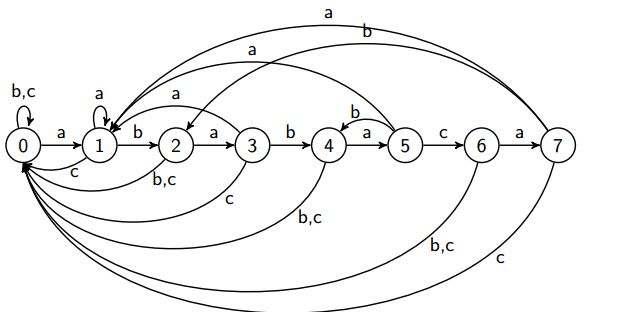
\includegraphics[scale=0.6]{fa.jpg}
\end{figure}
The only difference between the DFAs in CS 240 and the DFAs in CS 241 is that the DFAs in this course require a transition for \textit{every} possible character in our language.\\We say there there are $m$ states.
\subsubsection{State Transition}
To formally define a transition, we define the transition function $\delta$, which takes input of a state $q$ and a character $c$ in $\Sigma$:
$$\delta(q, c) = \ell(P[0..q-1]c)$$
where
\begin{itemize}
\item $P[0..q-1]c$ is the concatenation of $P[0..q-1]$ and $c$
\item for a string $s$, $\ell(s) \in \{0, \cdots, m\}$ is the length of the longest prefix of $P$ that is also a suffix of $s$
\end{itemize}
\begin{ex}
Consider the pattern $P = ababaca$ with $P[0..q] = aba$
\end{ex}
$$\delta(3, a) = \ell(abaa) = 1$$
$$\delta(3, b) = \ell(abab) = 4$$
$$\delta(3, c) = \ell(abac) = 0$$
%END%
\end{document}